\begin{figure}[htbp]
\centering
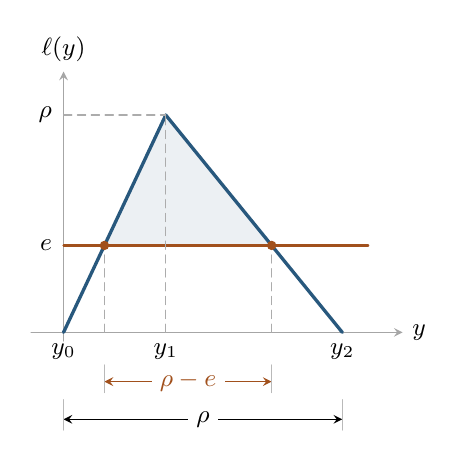
\begin{tikzpicture}[x=1.18cm,y=.92cm,font=\small,
  line cap=round,line join=round,>=stealth]
  \definecolor{sliceblue}{RGB}{40,88,125}
  \definecolor{sliceorange}{RGB}{161,80,28}
  \fill[sliceblue!9] (.44,1.2)--(1.1,3)--(2.24,1.2)--cycle;
  \draw[->,gray!70] (-.35,0)--(3.65,0) node[right,text=black] {$y$};
  \draw[->,gray!70] (0,-.12)--(0,3.6) node[above,text=black] {$\ell(y)$};
  \draw[sliceblue,very thick] (0,0)--(1.1,3)--(3,0);
  \draw[densely dashed,gray!65] (0,3)--(1.1,3);
  \draw[sliceorange,thick] (0,1.2)--(3.28,1.2);
  \draw[densely dashed,gray!65] (.44,0)--(.44,1.2)
    (2.24,0)--(2.24,1.2) (1.1,0)--(1.1,3);
  \fill[sliceorange] (.44,1.2) circle (1.7pt) (2.24,1.2) circle (1.7pt);
  \node[left,inner sep=4pt] at (0,3) {$\rho$};
  \node[left,inner sep=4pt] at (0,1.2) {$e$};
  \node[below,inner sep=4pt] at (0,0) {$y_0$};
  \node[below,inner sep=4pt] at (1.1,0) {$y_1$};
  \node[below,inner sep=4pt] at (3,0) {$y_2$};
  \draw[<->,sliceorange] (.44,-.68)--(2.24,-.68)
    node[midway,fill=white,inner sep=3pt] {$\rho-e$};
  \draw[gray!55] (.44,-.45)--(.44,-.83) (2.24,-.45)--(2.24,-.83);
  \draw[<->] (0,-1.20)--(3,-1.20)
    node[midway,fill=white,inner sep=3pt] {$\rho$};
  \draw[gray!55] (0,-.93)--(0,-1.35) (3,-.93)--(3,-1.35);
\end{tikzpicture}
\caption{Horizontal slice lengths of a triangle of area $\rho^2/2$
and vertical range $\rho$. The tent has height $\rho$. For
$0\le e\le\rho$, the heights in the vertical projection at which
$\ell(y)\ge e$ form an interval of length $\rho-e$.
The graph shows three distinct vertex heights; a horizontal side gives
the same conclusion with a one-sided tent.}
\label{fig:triangle-slices}
\end{figure}
